\chapter{Preliminaries}\label{C:soa}
\gls{rl} is intuitively describable as the process of learning from interaction with the environment. This hasty explanation offers a very high level definition of it, then a more formal way to model the problem is required to properly analyze it. To this end, this chapter provides a description of the mathematical framework required to model \gls{rl}. It also explains a selection of algorithms that are related to the work done in this thesis in order to provide enough knowledge about the literature I dealt with during my years of Ph.D. research.

\section{Agent and environment}
\begin{figure}[b]
\begin{minipage}{\textwidth}
\begin{center}
  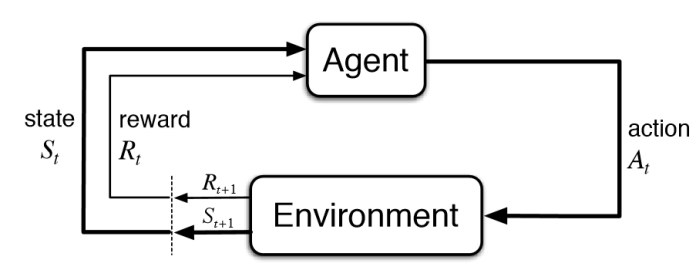
\includegraphics[scale=.75]{img/mdp1.jpg}
\end{center}
\end{minipage}
\caption[Reinforcement Learning problem scheme]{The scheme of a \gls{rl} model.}\label{F:mdp1}
\end{figure}
The interaction of an agent inside an environment can be seen as the execution of actions to move itself and the observation of the consequences of its actions (Figure \ref{F:mdp1}). The temporal progress of the interaction is modeled in a set of discrete time steps $t \in [0, 1, 2, \dots]$ where the agent sees a representation $s$ of the environment, executes an action $a$ and observes the new representation of the environment $s'$. The problems about observation and interaction discussed in Chapter~\ref{C:intro} are simplified by an explicit selection of data to observe from the environment and of the executable actions. In this way, only the relevant aspects of the sensory data acquired from the environment by the agent are used. The total number of time steps $t_i$ is called \textit{horizon} $H$ and determines a first taxonomy of problems:
\begin{itemize}
 \item finite time horizon: $t_i, \forall i \in [0, 1, 2, \dots, H)$;
 \item infinite time horizon: $t_i, \forall i \in [0, 1, 2, \dots, \infty)$.
\end{itemize}
Some problems can terminate before reaching the horizon, which happens when the agent reaches special situations called \textit{absorbing} states. These states are usually desired or catastrophic states when the interaction of the agent with the environment is no more useful or impossible. The set of steps between the start of the interaction to the end is called \textit{episode}.

The interaction of the agent with the environment is performed with the purpose to reach a goal for which the agent has been designed. The way to give the knowledge of the goal to the agent is to provide it with a measure of the quality of its behavior. This measure is called \textit{reward} $R(s,a,s')$ and is a function usually returning a real scalar value $r$ given the action $a$ performed by the agent in state $s$ and bringing to state $s'$. The goal of the agent is to maximize a measure related to the collected rewards. In an infinite time horizon problem it can be:
\begin{itemize}
 \item cumulative reward:
 \begin{equation}\label{E:sumrew}
  J = \sum_{t=0}^\infty r_t;
 \end{equation}
\item average reward:
\begin{equation}
 J = \lim_{n\to\infty}\dfrac{\sum_{t=0}^n r_t}{n};
\end{equation}
\item discounted cumulative reward:
\begin{equation}\label{E:discumrew}
 J = \sum_{t=0}^\infty \gamma^t r_t.
\end{equation}
\end{itemize}
The measure in Equation~\ref{E:discumrew} uses a real scalar $\gamma \in (0, 1]$, called \textit{discount factor}, which has the purpose to give different importance to rewards w.r.t. the time step they have been collected. If $\gamma = 1$ the equation reduces to~\ref{E:sumrew}, whereas the smaller it becomes the less the agent cares about rewards far in time.

\section{Markov Decision Processes}
\begin{figure}[t]
\begin{minipage}{\textwidth}
\begin{center}
  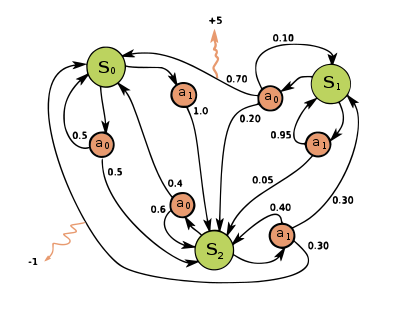
\includegraphics[scale=.6]{img/mdp2.png}
\end{center}
\end{minipage}
\caption[Markov Decision Process]{An example of a MDP graph representing states $S_i$, actions $a_i$, transition probabilities (numbers over each edge) and rewards (pink arrows).}\label{F:mdp2}
\end{figure}
The mathematical framework to study the interaction of the agent with the environment is provided by the theory behind \glspl{mdp}. A \gls{mdp} is defined as a $6$-tuple where $\langle \mathcal{S}, \mathcal{A}, \mathcal{R}, \mathcal{T}, \gamma, \mu \rangle$:
\begin{itemize}
 \item $\mathcal{S}$ is the set of states where the agent can be in the environment;
 \item $\mathcal{A}$ is the set of actions that the agent can execute in the environment;
 \item $\mathcal{R}$ is the set of rewards obtainable by the agent;
 \item $\mathcal{T}$ is the \textit{transition function} consisting in the probability of reaching a state $s'$ executing action $a$ in state $s$: $\mathcal{T}(s, a) = P(s' | s, a)$;
 \item $\gamma$ is the discount factor;
 \item $\mu$ is the probability of each state to be the initial one: $\mu(s) = P(s_0 = s)$.
\end{itemize}
A \gls{mdp} is called \textit{finite}, or \textit{discrete}, if the set of states $\mathcal{S}$ and set of actions $\mathcal{A}$ are finite; it is called \textit{infinite}, or \textit{continuous}, when the set of states $\mathcal{S}$ is infinite and/or the set of actions $\mathcal{A}$ is infinite.
Two important properties of \glspl{mdp} are:
\begin{itemize}
 \item \textbf{stationarity:} the transition function $\mathcal{T}$ does not change over time;
 \item \textbf{Markovian assumption:} the transition and reward function depend only on the current time step and not on the previous ones;
 \item \textbf{ergodicity:} a \gls{mdp} is called \textit{ergodic} when the agent can reach all the states of the \gls{mdp} from every state.
\end{itemize}
These three properties are taken as assumptions by most of the literature about \glspl{mdp} and by the works presented in this thesis too.

\subsection{Value functions}
Recalling that the goal of the agent is to maximize the cumulative (discounted) reward $J$ obtained during an episode, a \gls{mdp} is considered \textit{solved} when the agent learns the actions to perform in each state which maximizes this measure. The function defining the probability of executing action $a$ in a state $s$ is called \textit{policy}: $\pi(s) = P(a|s)$. An \textit{optimal} policy $\pi^*$ is the one which, when followed, allows the agent to solve the \gls{mdp}. Considering the stochasticity in the transition function $\mathcal{T}$ and in the policy $\pi$, the expected value of the cumulative discounted reward obtainable following $\pi$ is called \textit{state-value function}
\begin{equation}
 V_\pi(s) = \mathbb{E}_\pi[\sum_{k=0} \gamma^k r_{t+k}], \forall s \in \mathcal{S}.
\end{equation}
Then, an optimal policy can be defined also as the one which maximizes the value function of each state
\begin{equation}
 V^*(s) = \max_\pi V_\pi(s), \forall s \in \mathcal{S}.
\end{equation}
Together with the state-value function, the \textit{action-value function} is defined as
\begin{equation}
 Q_\pi(s, a) = \mathbb{E}_\pi[\sum_{k=0} \gamma^k r_{t+k}], \forall s \in \mathcal{S}, a \in \mathcal{A}.
\end{equation}
And subsequently the optimal policy maximizes also the action value function of each state-action tuple
\begin{equation}
 Q^*(s,a) = \max_\pi Q_\pi(s,a), \forall s \in \mathcal{S}, a \in \mathcal{A}.
\end{equation}

\section{Solving a MDP}
Value functions are the main concept used by several algorithms to address the problem of solving \glspl{mdp}. In the following, a description of algorithms exploiting value functions to solve \glspl{mdp} is provided, from the easiest case to the hardest ones.

\subsection{Dynamic Programming}
When the transition function $\mathcal{T}$ and reward function $\mathcal{R}$ of a \gls{mdp} are known, the full model of the environment is available. This is not the case in many real world problems where an agent does not know where the action would bring it and which return would obtain, but constitutes an interesting scenario to start studying the problem of solving a \gls{mdp}. The theory behind the solving of \glspl{mdp} with full model available is known under the name of \gls{dp}~\cite{bertsekas2005dynamic, bellman2013dynamic}. The main concept in the research on \gls{dp} is the optimal \gls{be}, defined as
\begin{align}
 V^*(s) &= \max_a \mathbb{E}[r_t + \gamma V^*(s')]\nonumber\\
        &= \max_a \sum_{s'} p(s' | s, a)[r + \gamma V^*(s')]
\end{align}
for state-value function, and
\begin{align}
 Q^*(s,a) &= \mathbb{E}[r_t + \gamma \max_{a'}Q^*(s', a')]\nonumber\\
          &= \sum_{s'} p(s' | s, a)[r + \gamma \max_{a'}Q^*(s', a')]
\end{align}
for action-value function $\forall (s, s') \in \mathcal{S} \times \mathcal{S}$ and $a \in \mathcal{A}$.
The optimal \gls{be} serves as a way to derive the optimal policy, but requires the optimal value functions to be known. Usually the optimal value functions are unknown and in order to learn them several algorithms change the \gls{be} in form of an assignment repeated iteratively.

\subsubsection{Policy Iteration}
The iterative application of the \gls{be} when following a policy $\pi$ is called \textit{iterative policy evaluation} (Algorithm~\ref{A:peval}) since it allows to compute the value functions of states and actions w.r.t. the policy $\pi$:
\begin{align}
 V_{t+1} (s) &= \mathbb{E}_\pi[r_t + \gamma V_t(s_{t+1})]\nonumber\\
             &= \sum_a \pi(a|s) \sum_s P(s' | s, a)[r + \gamma V_t(s')], \forall s \in \mathcal{S}. 
\end{align}
\begin{algorithm}[t]
 \caption{Iterative Policy Evaluation}
 \begin{algorithmic}[1]\label{A:peval}
  \STATE \textbf{Inputs:} policy $\pi$ to evaluate, a small threshold $\theta$ determining the accuracy of the estimate
  \STATE \textbf{Initialize:} $V(s), \forall s \in \mathcal{S}$ arbitrarily, $V(s') = 0$ for all terminal states $s'$
  \REPEAT
  \STATE $\Delta \gets 0$
  \FORALL{$s \in \mathcal{S}$}
  \STATE $v \gets V(s)$
  \STATE $V(s) \gets \sum_a \pi(a|s) \sum_{s'} P(s'|s,a)[r + \gamma V(s')]$
  \STATE $\Delta \gets \max(\Delta, |v - V(s)|)$
  \ENDFOR
  \UNTIL{$\Delta < \theta$}
 \end{algorithmic}
\end{algorithm}
It can be shown that the iterative application of the \gls{be} always converges to a single fixed point $V_\pi$.

Once the value functions have converged, it is interesting to see if the current policy $\pi$ can be improved in order to make it closer to the optimal one $\pi^*$ or not. One way to do this consists in considering a state $s$ and an action $a \neq \pi(s)$ and computing
\begin{align}
 Q_\pi(s,a) &= \mathbb{E}[r_t + \gamma V_\pi(s_{t+1})]\nonumber\\
            &= \sum_{s'} P(s' | s,a)[r + \gamma V_\pi(s')], \forall s \in \mathcal{S}, a \in \mathcal{A}.
\end{align}
Whenever $Q_\pi(s,a) > Q_\pi(s, \pi(s))$ it is convenient to update the policy such as $\pi(s) = a$. This procedure is called \textit{policy improvement}.
The process of alternating steps of iterative policy evaluation and policy improvement brings to the estimation of the optimal value functions and is resumed in an algorithm called \gls{pi} (Algorithm~\ref{A:piter}).
\begin{algorithm}[t]
 \caption{Policy Iteration}
 \begin{algorithmic}[1]\label{A:piter}
  \STATE \textbf{Initialize:} $\pi(s) \in \mathcal{A}$ arbitrarily for all $s \in \mathcal{S}$
  \REPEAT
  \STATE \textbf{Iteration policy evaluation}
  \STATE \textbf{Policy improvement:}
  \STATE $policy\_stable \gets true$
  \FORALL{$s \in \mathcal{S}$}
  \STATE $old\_a \gets \pi(s)$
  \STATE $\pi(s) \gets arg\max_a \sum_{s'} P(s'|s,a)[r + \gamma V(s')]$
  \STATE If $old\_a \neq \pi(s)$, then $policy\_stable \gets false$
  \ENDFOR
  \UNTIL{policy-stable}
 \end{algorithmic}
\end{algorithm}

\begin{algorithm}[t]
 \caption{Value Iteration}
 \begin{algorithmic}[1]\label{A:viter}
  \STATE \textbf{Inputs:} a small threshold $\theta$ determining the accuracy of the estimate
  \STATE \textbf{Initialize:} $V(s), \forall s \in \mathcal{S}$ arbitrarily, $V(s') = 0$ for all terminal states $s'$
  \REPEAT
  \STATE $\Delta \to 0$
  \FORALL{$s \in \mathcal{S}$}
  \STATE $v \to V(s)$
  \STATE $V(s) \to \max_{a} P(s'|s,a)[r + \gamma V(s')]$
  \STATE $\Delta \gets \max(\Delta, |v - V(s)|)$
  \ENDFOR
  \UNTIL{$\Delta < \theta$}
 \end{algorithmic}
\end{algorithm}

\subsubsection{Value Iteration}
The alternation of policy evaluation and policy improvement is a drawback of \gls{pi} which may slowdown the learning. Among other algorithms, the algorithm of \gls{vi} (Algorithm~\ref{A:viter}) addresses this problem stopping policy evaluation after only one update of each state value function. The update is different from the one in policy evaluation since it combines the policy evaluation steps and the policy improvement:
\begin{align}
 V_{t+1} (s) &= \max_a \mathbb{E}[r_t + \gamma V_t(s_{t+1})]\nonumber\\
             &= \max_a \sum_s P(s' | s, a)[r + \gamma V_t(s')], \forall s \in \mathcal{S}. 
\end{align}
Desirably, \gls{vi} maintains the properties of \gls{pi} about convergence to the fixed point corresponding to the optimal value functions.

As stated at the beginning of the section, the previous methods can be applied only when the full model of the \gls{mdp} is known. However, in most of real cases the full model is not available and the agent must move in the environment in order to understand it.

\subsection{Reinforcement Learning}
The purpose of \gls{rl} is to address the problem of solving a \gls{mdp} in the cases where \gls{dp} is not helpful, i.e. when the transition function $\mathcal{T}$ and reward function $\mathcal{R}$ are not known. To achieve this, the agent should acquire the necessary knowledge from transition samples obtained moving in the environment. There are two main ways of using the transition samples resulting in two classes of \gls{rl} algorithms:
\begin{itemize}
 \item \textbf{model-based:} the samples are used to learn a model of the environment which is subsequently used to learn the policy;
 \item \textbf{model-free:} the samples are used to directly compute the policy, for instance by means of value function approximation.
\end{itemize}
In both classes of methods, the \gls{rl} problem can be addressed in two ways:
\begin{itemize}
 \item \textbf{value-based:} the algorithm computes an estimate of the action-value function;
 \item \textbf{policy-based:} the algorithm computes an estimate of the policy.
\end{itemize}
This taxonomy splits the \gls{rl} literature in two sharply different fields where value-based is mostly used for discrete \glspl{mdp} whilst policy-based is mostly used in continuous \glspl{mdp}, in particular in Robotics~\cite{kober2013reinforcement}.

In all these classes of problems the policy followed to collect samples plays a crucial role since the performance of the learning algorithm heavily depends on the balancing between exploratory actions and exploitative actions, a fundamental issue of \gls{rl} known as \textit{exploration-exploitation dilemma}. The work done in this thesis is mainly focused on model-free value-based \gls{rl} in \gls{mdp} with a finite number of actions, thus all the following analysis is only inherent to it.

\paragraph{Exploration policies}
In a hypothetical setting in which the agent is provided the knowledge of the optimal policy $\pi^*$, there is no need to explore new actions and it can simply follow the optimal policy to solve the \gls{mdp} even without learning anything. Besides this very unlikely case, there are numerous situations where the agent does not know the environment it is moving in and the effect of its actions on the environment, then it needs to explore the environment to acquire the knowledge it needs to learn an optimal policy. The most trivial exploratory policy is called $\varepsilon$-greedy and is computed as
\begin{equation}\label{E:eps}
\pi(a|s)=
    \begin{cases}
    \dfrac{\varepsilon}{|\mathcal{A}|} + 1 - \varepsilon & \text{if } a = \arg\max_{a \in \mathcal{A}}Q(s,a)\\
    \dfrac{\varepsilon}{|\mathcal{A}|} & \text{otherwise}
    \end{cases}
\end{equation}
Equation~\ref{E:eps} results in choosing, at each step, between a greedy or a random action according to the value of $\varepsilon$: the policy is completely random when $\varepsilon = 1$ and is completely greedy when $\varepsilon = 0$.
Despite its simplicity, this policy is used in numerous works in literature allowing to reach good results with minimum computational demand, but at the cost of a bad sample-efficiency.

One of the drawbacks of $\varepsilon$-greedy is that it makes no use of the information available to the agent. The \textit{Boltzmann} policy, also known as \textit{Softmax} policy, makes use of the current estimate of the action-value functions computing the probabilities for each action $a_i$ to be sampled as
\begin{equation}\label{E:boltz}
 \pi(a | s) = \dfrac{e^{\nicefrac{Q(s,a)}{\tau}}}{\sum_{a' \in \mathcal{A}}e^{\nicefrac{Q(s,a')}{\tau}}}
\end{equation}
where $\tau$ is called \textit{temperature} and controls the exploration ratio such as if $\tau \to 0$ the policy is greedy and if $\tau \to \infty$ the policy is random. This is an attempt to use knowledge acquired by the agent in order to drive exploration in a smarter way than $\varepsilon$-greedy. A more recent strategy based on Boltzmann policy exploits the \gls{mm} operator to compute the Maximum Entropy \gls{mm} policy~\cite{asadi2016alternative}
\begin{equation}
 \pi(a | s) = \dfrac{e^{\nicefrac{Q(s,a)}{\tau}}}{\sum_{a' \in \mathcal{A}}e^{\nicefrac{Q(s,a')}{\tau}}}
\end{equation}
where $\beta$ is a value for which
\begin{equation}
 \sum_{a \in \mathcal{A}} e^{\beta(Q(s,a) - mm_\omega Q(s))}(Q(s,a)-mm_\omega Q(s))=0
\end{equation}
and
\begin{equation}\label{E:mm}
 mm_\omega Q(s) = \dfrac{\log(\dfrac{\sum_{i=1}^{|\mathcal{A}|}e^{\omega Q(s,a_i)}}{|\mathcal{A}|})}{\omega}.
\end{equation}
The \gls{mm} operator~\ref{E:mm} is a softmax operator with the desirable property of differentiability of the Boltzmann operator~\ref{E:boltz}, but differently from the Boltzmann it is also a contractive operator, thus being an interesting operator for computing the target of the \gls{be}. 

\subsubsection{Temporal Difference Learning}
Given a policy, \gls{rl} is able to evaluate it from raw experience differently from \gls{dp} which needs to know the complete model of the \gls{mdp}. A well-known class of methods to do this is called \gls{mc}~\cite{robert2013monte} and consists in collecting samples for an entire episode and then updating the considered value functions using the discounted cumulative reward obtained during the run:
\begin{equation}\label{E:mc}
 V(s) \gets V(s) + \alpha [G - V(s)]
\end{equation}
where $G$ is the cumulative reward obtained from state $s$ till the end of the episode and $\alpha$ is the learning rate.
The drawback of these techniques is that they need the episode to be finished before updating the value function estimates slowing down the learning time.

To keep the desirable property of \gls{mc} of being able to estimate value functions from raw experience without losing the good property of \gls{dp} of being able to update the same estimates after each step (i.e. \textit{bootstrapping}), \gls{td} methods have been studied in the past literature and are still one of the most used methods in \gls{rl}. The simplest \gls{td} method is known as \gls{td}$(0)$ and updates the value function after each step with
\begin{equation}
 V(s) \gets V(s) + \alpha [r + \gamma V(s') - V(s)].
\end{equation}
The success of \gls{td} over \gls{dp} and \gls{mc} is motivated by this simple update formula since the algorithm is able to take the advantages of both techniques with guarantees of convergence to the optimal value function.

\gls{td} methods can be used for control if, instead of computing the state-value function, the action-value function is computed. This class of methods is split in two subclasses according to which policy is followed to compute the target of the \gls{td} update:
\begin{itemize}
 \item \textbf{on-policy:} following the policy which the agent is learning;
 \item \textbf{off-policy:} following another policy.
\end{itemize}

\paragraph{SARSA}\label{S:SARSA}
The SARSA algorithm is a well-known on-policy TD method for control. Being an on-policy control method, given a policy $\pi$ its purpose is to estimate the action-value function $Q_\pi(s,a)$ for each $(s,a)$ tuple via the update formula:
\begin{equation}
 Q(s,a) \gets Q(s,a) + \alpha [r + \gamma Q(s',a') - Q(s,a)]
\end{equation}
where $a' = \pi(s')$. Being a \gls{td}$(0)$ variant for control, the same convergence properties of \gls{td}$(0)$ apply for SARSA.
\paragraph{$Q$-Learning}\label{S:Q-Learning}
The corresponding off-policy \gls{td} algorithm for control w.r.t. SARSA is \gls{ql}~\cite{watkins1989learning}. Contrarily to SARSA, \gls{ql} directly approximates the optimal action-value functions using a different policy to compute the target of the \gls{td} update. In particular, \gls{ql} uses the greedy policy to compute the target, resulting in the update formula
\begin{equation}\label{eq:Q-formula}
 Q(s,a) \gets Q(s,a) + \alpha_t(s,a) \left(r + \gamma \max_{a'} Q(s',a') - Q(s,a)\right).
\end{equation}

According to the difference between on-policy and off-policy methods, SARSA and \gls{ql} are two algorithms that may behave very differently in some problems where the agent can reach some catastrophic states. For instance, if the desired goal state is close to other undesirable catastrophic states, SARSA will learn a policy which let the agent stay far to undesired state and reach the goal safely but slowly; while \gls{ql} will learn a policy moving close to undesired states, but reaching the goal faster than SARSA. Thus, SARSA is more suitable for real applications, e.g. in Robotics, where the cost of reaching catastrophic situations is very high and is better to be conservative in order not to damage the physical system; on the contrary, \gls{ql} is more suitable when the cost of reaching bad states is not high, e.g. simulations.

\paragraph{Fitted Q-Iteration}\label{S:FQI}
A well known \gls{td} batch variant of $Q$-Learning is the \gls{fqi} algorithm~\cite{ernst2005tree}. The idea of \gls{fqi} is to reformulate the \gls{rl} problem as a sequence of supervised learning problems. Given a set of samples $\mathcal{D} = \left\{\langle s_i, a_i, r_i, s'_i \rangle \right\}_{1\leq i\leq N}$ previously collected by the agent according to a given sampling strategy, at each iteration $t$, \gls{fqi} builds an approximation $\hat{Q}$ of the optimal $Q$-function by fitting a regression model on a bootstrapped sample set
\begin{equation}
 \mathcal{D}_t = \left\{ \langle (s_i,a_i), r_i + \gamma \max_{a'} \hat{Q}\left(s'_i, a'\right) \rangle\right\}_{1 \leq i \leq N}.
\end{equation}
Under some conditions, the algorithm is proved to converge to the optimal $Q$ in a finite number of steps. \gls{fqi} has been firstly presented using extra-trees regression~\cite{geurts2006extremely}, but has been proved to work well with other kind of regression, e.g. neural network in the \gls{nfqi} algorithm~\cite{riedmiller2005neural} or \gls{gp} regression~\cite{rasmussen2005gaussian} in the Weighted Fitted Q-Iteration algorithm~\cite{deramo2017maximum}.

\subsubsection{Deep Reinforcement Learning}
The groundbreaking works that revived the research on \gls{rl} in recent years are certainly the ones belonging to the \gls{drl} field which consists to the use of \gls{dl} methodologies to address the \gls{rl} problem in complex high-dimensional \glspl{mdp}. Indeed, the very large state and action spaces together with the high number of features represent an obstacle to the learning with shallow \gls{rl} techniques making them computationally impractical. The recent coming of powerful computational resources, in particular the use of \glspl{gpu} for training deep neural networks in \gls{dl}, allowed to overcome this issue favoring the use of powerful deep function approximators in \gls{rl}.

\paragraph{Deep Q-Network}\label{S:dqn}
\begin{figure}[t]
\begin{minipage}{\textwidth}
\begin{center}
  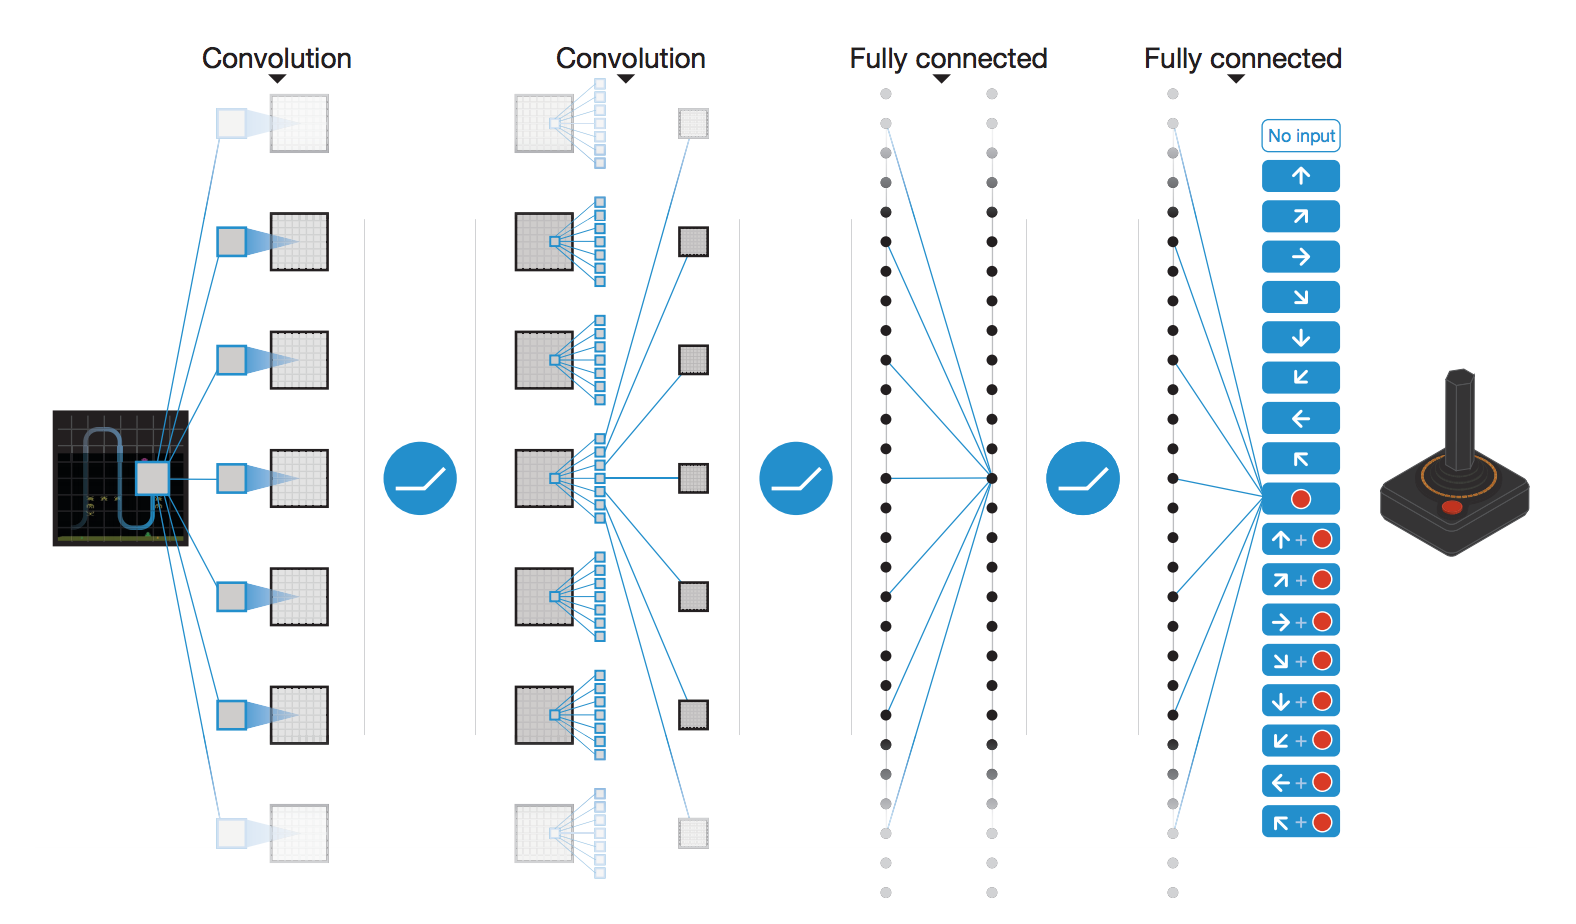
\includegraphics[scale=.19]{img/dqn.png}
\end{center}
\end{minipage}
\caption[DQN network scheme]{Synthetic scheme of a deep neural network which takes the input of the screen of a videogame and outputs the action to perform in that state.}
\end{figure}
The pioneering work which showed the potential of \gls{drl} and started the research about it is the \gls{dqn} algorithm~\cite{mnih2015human}. It consists in the use of a deep neural network and the storing of a replay memory of past transitions $\langle s_t, a_t, r_t, s'_t \rangle$ to approximate the action-value function $\hat{Q}$ of the problem computing the target
\begin{equation}\label{E:dqn_update}
y_i=
    \begin{cases}
    r_i & \text{if episode terminates at episode }i+1\\
    r_i + \gamma \max_{a'} \hat{Q}(s'_i, a') & \text{otherwise}
    \end{cases}
\end{equation}
and learning it in a supervised way.

The algorithm shows outstanding performance on the previously almost intractable problems of Atari games~\cite{bellemare2013arcade}, a set of more than $50$ old but challenging videogames, where \gls{dqn} achieves state-of-the-art results even beating a human expert in some of them. The most remarkable quality of \gls{dqn} is its relatively simple implementation consisting of using raw pixel frame as input of a convolutional network and applying a simple gradient descent step to update the network. In this way the complexity of the input, that made the solving of these problems intractable in the past, is addressed with the power of the deep convolutional network to extract highly abstract representation of it sensibly reducing its dimensionality and making it suitable for approximating the action-value function effectively. Despite its good properties, \gls{dqn} has some issues about sample-efficiency and the stability of learning that are common problems among \gls{drl} techniques. Indeed, the number of samples required by \gls{dqn} to learn are in the order of millions and corresponds to more than month of human playing; moreover in some games the algorithm shows very unstable performance even bringing to completely forgetting the good policy it learned after many steps. For these reasons, without forgetting the promising line of research that \gls{dqn} revealed, the following literature focused on many variants of \gls{dqn} to improve some of the issues it has. For instance, Double DQN~\cite{hasselt2015double} has been proposed to improve the estimate of the action-value function whereas Bootstrapped DQN~\cite{osband2017deep} aims to improve the exploration capabilities; both these algorithms will be considered and explained further in the thesis respectively in Chapter~\ref{C:mev} and~\ref{C:ts}.
